\section{What is a Genetic Algorithm?}
\begin{figure}[h]
	\centering
		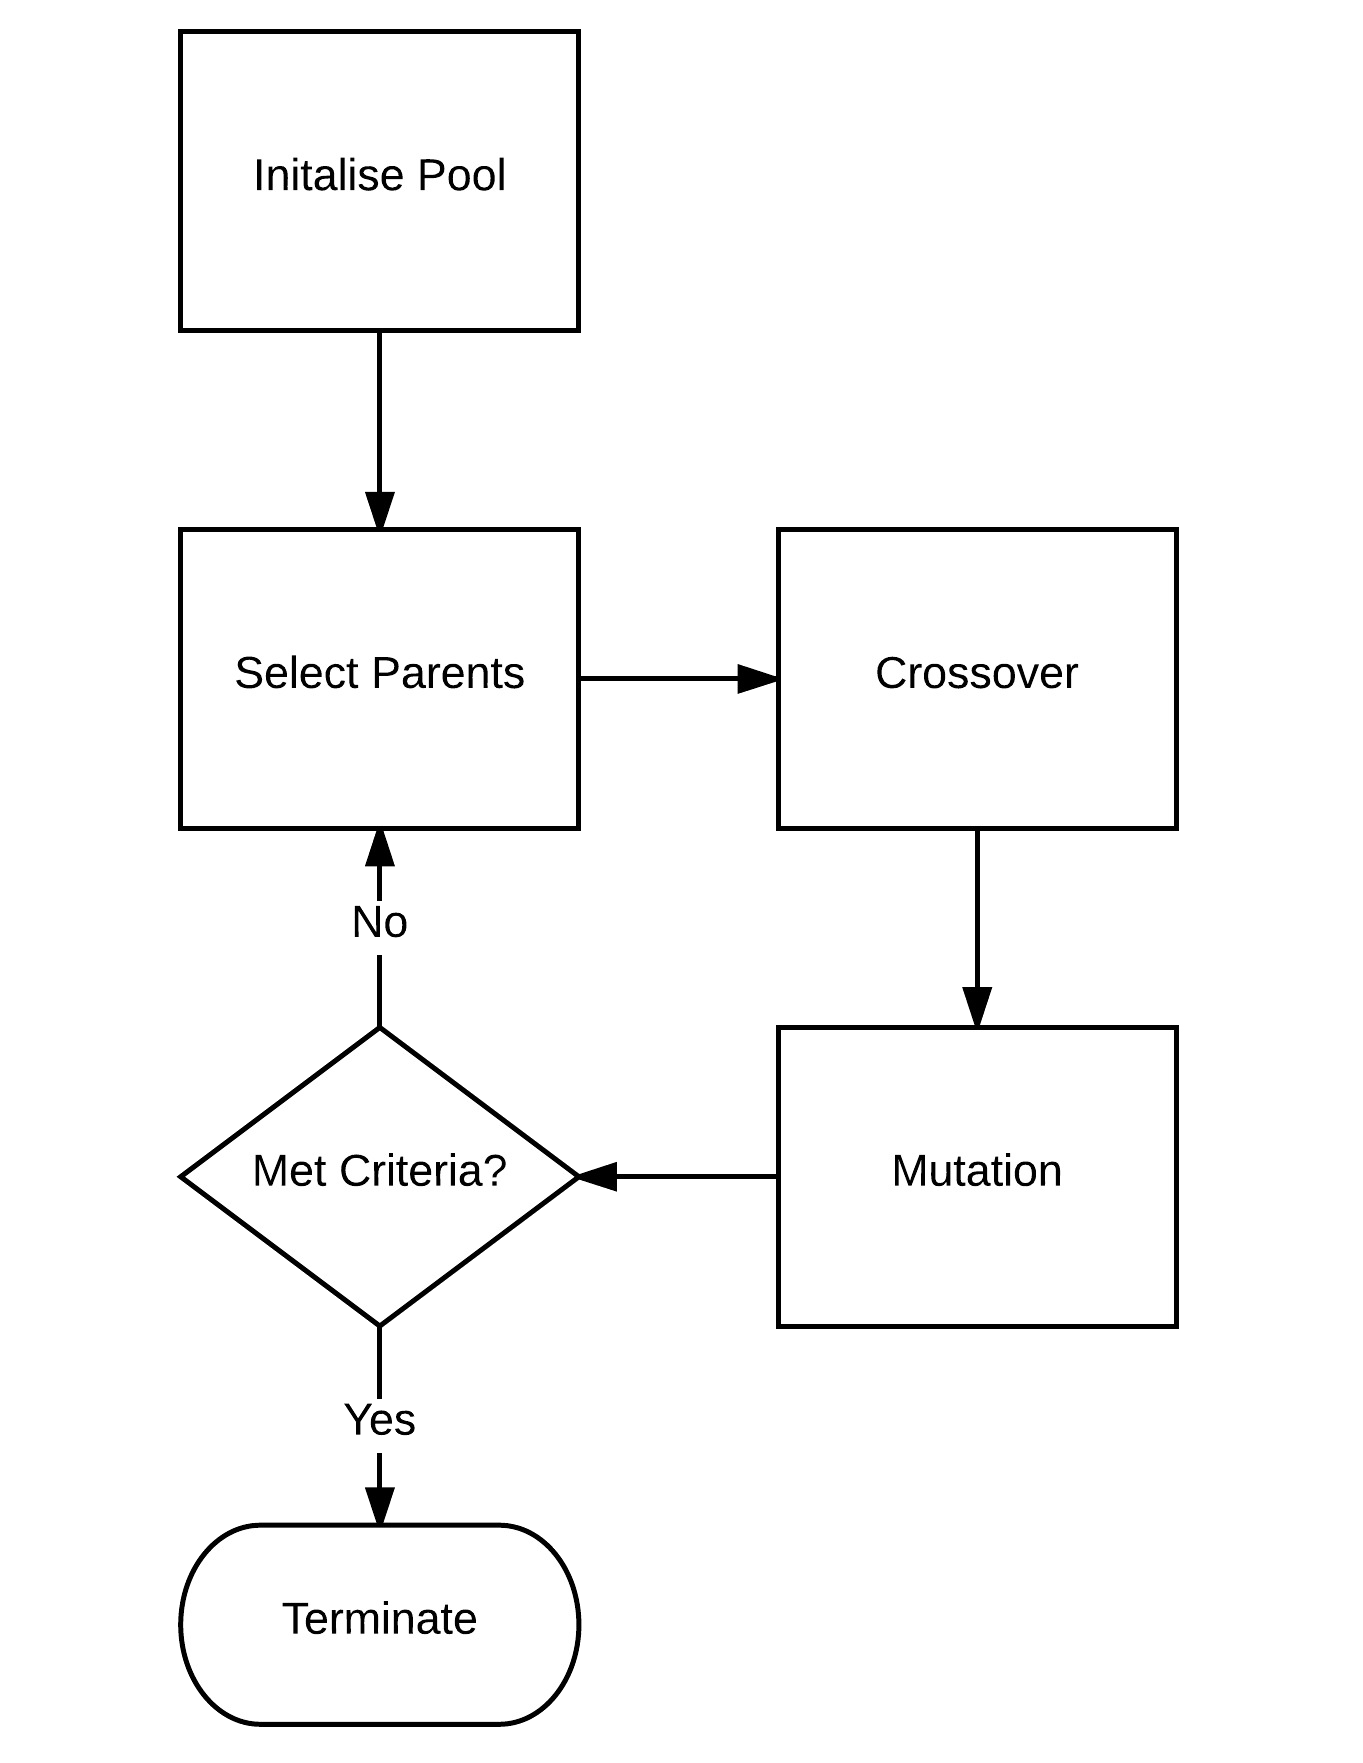
\includegraphics[width=0.5\textwidth]{GA_Structure}
	\caption{The basic structure of a Genetic Algorithm.}
	\label{struct}
\end{figure}
\noindent
A Genetic Algorithm is an algorithm that uses natural selection, or survival of the fittest, to find a solution to a problem. All Genetic Algorithms follow a similar, if not identical structure (figure \ref{struct}). However, the elements of this structure are highly customised for each specific application. Before going into detail about these elements, the concept of chromosomes and fitness must first be introduced.
\par
Chromosomes are one of the most important part of a GA, their only purpose is to store the potential solutions of the problem. How chromosomes store these solutions is up to the constructor of the GA, commonly however they are a single string that might represent a binary number, or possibly a list of the problems variables. Another important thing about chromosomes is their fitness. The fitness function of a GA describes how fit a particular problem is as a solution. How this fitness works, and how fitnesses are compared is again nearly entirely up to the constructor of the GA.


\section{Initialisation of the Pool}
\par
The first step in the execution of a Genetic algorithm is the generation of the pool. The pool is a collection of chromosomes that can be described as the "current generation". This pool is initialised by randomly generating chromosomes until the pool is filled, in the case of the research algorithm, this was done by shuffling the list of cities, thus eliminating the possibility of missing or having duplicate cities within the chromosome. The number of chromosomes in the pool is usually a fixed number, however adaptive pool sizing does exist (http://www.sciencedirect.com/science/article/pii/S2212671613000449) only fixed pool size was used in this research. 
\section{The Main Loop}
\par
This next section comprises the main body of the GA. Every time this loop is completed, a generation has passed. Through out the next sections, the methods used in the research algorithm will be used as examples.
\subsection{Parent Selection}
\par
Parent selection is the first step of each generation. The flow of Figure \ref{struct} suggests that all parents are selected before Crossover, however in reality it is easier and potentially more efficient to do both steps concurrently, thus you select two parents, breed them (Crossover) and repeat until a new pool is constructed.
\par
Parents can be selected in many ways, however usually the fitness of the parents is used in some way to select them. For example, in the research algorithm a method called roulette wheel selection was used (INSERT SOME REFERENCE HERE), in this method all chromosomes in the pool take up an area on a wheel proportional to the fitness of the chromosome. This created some issues as within the research algorithm as the fitness function returns the total distance of the chromosome, thus the smaller that distance the better it is. In order to get the correct probability of selection, the fitnesses needed to be 'inverted'. This was done with two equations: 
\begin{figure}
\[ inv = minFit + maxFit\]
\caption{Where inv is the 'Inversion constant', minFit is the smallest/best fitness in the pool and maxFit is the largest/worst fitness in the pool.}
\end{figure}
\begin{figure}
\[ p = (inv - fitness)/totalInvFitness\]
\caption{Where p = the probability of selection, inv is the 'Inversion constant', fitness is the fitness of a chromosome, and totalInvFitness is the sum of all inverted fitnesses in the pool}
\end{figure}
Using these equations, the probability of selection for each chromosome in the pool could be calculated, thus allowing for parents to be randomly selected from the pool using these probabilities.
\subsection{Crossover}
\par
Crossover (also known as breeding) is when two chromosomes, called parents, are 'crossed' together in some way to produce one or more children. There are many ways of doing this, from slicing the parents in half and swapping the ends, to more complicated methods like the one used in the research algorithm that shall be presented now.

--insert Crossover images--

\subsection{Mutation}
\par
\section{Termination}
\par
\section{The Research Framework}
\par
The Genetic Algorithm that was constructed for this research -----

